\documentclass{article}
\usepackage{amssymb,amsmath}

\usepackage[spanish, activeacute]{babel}
\usepackage{theorem}
\usepackage{times}
\usepackage{array}
\usepackage{graphicx}
\usepackage{hyperref}
\usepackage{multirow}
\usepackage[cp1252]{inputenc}
\usepackage{hhline}
\usepackage{multicol}

\hyphenation{me-di-ble}
\renewcommand{\sin}{\hbox{sen }}

%===========================estilo teoremas=============================

\newcounter{ejer}

{\theorembodyfont{\rmfamily}
\newtheorem{ejercicio}[ejer]{Ejercicio}}

\renewcommand{\theenumi}{\alph{enumi}}

\begin{document}

\hyphenation{excen-tri-ci-dad}
 %%%%%%%%%Estilo de la pagina%%%%%%%%%%%%%%%%%%%%%%%%%%%%%%%%%%%
%%%%%%%%%%%%%%%%%%%%%%%%%%%%%%%%%%%%%%%%%%%%%%%%%%%%%%%%%%%%%%%%%%
\setlength{\unitlength}{1cm}
%
\setlength{\extrarowheight}{5mm}
%

\begin{tabular}{m{.2\textwidth} m{.7\textwidth}}\hline\hline

\includegraphics[scale=.5]{unrc.eps} &
\begin{large}
\begin{bfseries}  \begin{scshape}
Facultad de Cs. Exactas, Fco-Qcas y Naturales\par
        Depto de Matem\'atica.\par
        Primer Cuatrimestre de 2017\par
        Ecuaciones Difereniales. Cod. 1913 \par
        Pr�ctica 4: Existencia y Unicidad.

\end{scshape}
\end{bfseries}
\end{large}\\ \hline\hline
\end{tabular}

\begin{ejercicio}
Transformar los siguientes sistemas de ecuaciones de primer orden en una ecuaci�n de segundo orden.

\begin{itemize}

\item[a.]
\begin{equation*}
\left\{\begin{array}{cc}
x'(t)&=x^2(t)+y(t)\\
y'(t)&=x(t)+2y(t)
\end{array}\right.
\end{equation*}

\item[b.]
\begin{equation*}
\left\{\begin{array}{cc}
x'(t)&=x(t)+z(t)\\
y'(t)&=tx(t)-z(t)\\
z'(t)&=-t^2x(t)+y(t)
\end{array}\right.
\end{equation*}

\item[c.]
\begin{equation*}
\left\{\begin{array}{cc}
x'(t)&=x(t)y(t)\\
y'(t)&=x(t)-y(t)\\
\end{array}\right.
\end{equation*}

\end{itemize}

\end{ejercicio}


\begin{ejercicio}  Encontrar o demostrar que no existe una
constante de Lipschitz para las siguientes funciones en
los dominios indicados.
\begin{enumerate}
\item $f(t,x)=t|x|$, en $|t|<a$, $x\in\mathbb{R}^n$.
\item $f(t,x)=x^{1/3}$ en $|x|<1$.
\item $f(t,x)=\frac{1}{x}$ en $1\leq x<\infty$.
\item $f(t,x)=(x_1^2x_2,t+x_3,x_3^2)$ en $|t|\leq a$, $|x|\leq b$
\end{enumerate}
\end{ejercicio}




\begin{ejercicio}
Sea $A\in \mathbb{R}^{n\times n}$ y $x_{0}\in \mathbb{R}^{n}$. Considerar el sistema
\begin{equation}\label{ec3}
\left\{\begin{array}{cc}
x'(t)=A\cdot x(t) \\
x(0)=x_{0}.
\end{array}
\right.
\end{equation}
\begin{itemize}
\item[a.] Sea $y(t):\mathbb{R}\to\mathbb{R}^{n}$ continua, demostrar que 
\begin{equation*}
\int_0^t A\cdot y(s)ds=A\cdot\int_0^t y(s)ds.
\end{equation*}
\item[b.] Aplicar la iteraci�n de Picard con la funci�n de partida $\varphi_{0}(t)\equiv x_{0}$ y demostrar que 
\begin{equation*}
\varphi_{n}(t)=\left(\sum_{i=0}^{n}A^{i}\frac{t^i}{i!}\right)\cdot x_{0},
\end{equation*}
donde $A^i=\underset{i-\text{veces}}{\underbrace{A\cdots A}}$ y $A^0=I$.
\end{itemize}
\end{ejercicio}



\begin{ejercicio}
El movimiento escilatorio de una part�cula de masa $m$, que se encuentra en un extremo de un resorte, y este est� fijado a la pared, est� dado por la ecuaci�n
\begin{equation*}
mx''(t)=-kx(t),
\end{equation*}
donde $x(t)$ es la posici�n de la part�cula,  el origen de coordenadas est� en la posici�n de reposo de la masa cuando el resorte no est� estirado ni contra�do, y $k$ es la constante de elasticidad del resorte.

Para una part�cula que inicialmente est� en la posici�n $x(0)=0$ y se le da una velocidad inicial $x'(0)=1\frac{mts}{s}$ la funci�n que modela su movimiento resuelve el problema
\begin{equation}\label{ec1}
\left\{\begin{array}{cc}
mx''(t)=-kx(t) &  t\in [0,\infty)\\
x(0)=0\\
x'(0)=1.
\end{array}
\right.
\end{equation}
\begin{itemize}
\item[a.] Transformar el problema anterior a un sistema de ecuaciones de primer orden.
\item[b.] Aproximar la soluci�n con el m�todo de Picard. Tomar como funci�n inicial $\varphi_{0}\equiv (0,1)$ y comparar $\varphi_{n}$ con el polinomio de grado $n$ de la soluci�n de \eqref{ec1}.
\end{itemize}
\end{ejercicio}

\begin{ejercicio}
Considerar el problema
\begin{equation}\label{ec2}
\left\{\begin{array}{cc}
x''(t)+2x'(t)+x(t)=0\\
x(0)=0\\
x'(0)=1.
\end{array}
\right.
\end{equation}
\begin{itemize}
\item[a.] Transformar la ecuaci�n de segundo orden en un sistema de ecuaci�nes de primer orden y obtener un problema a valores iniciales de primer orden.
\item[b.] Aplicar el m�todo de Picard al problema obtenido en el �tem \textrm{a}, tomando como funci�n inicial $\varphi_{0}\equiv(0,1)$ y demostrar que, para $n\geq 1$, $$\varphi_{n}(t)=\left(t\sum_{i=0}^{n-1}(-1)^{i}\frac{t^{i}}{i!},\sum_{i=0}^{n}(-1)^{i}(i+1)\frac{t^{i}}{i!}\right)$$. 
\item[c.] Utilizar el resultado obtenido en el �tem \textrm{b} para demostrar que $te^{-t}$ es la soluci�n de \eqref{ec2}.
\end{itemize}
\end{ejercicio}










\begin{ejercicio}   Sea $f:\mathbb{R}^2\to\mathbb{R}$ definida por
$f(t,x)=\sqrt{|x|}$. Consideremos el PVI:
\[
    \left\{%
\begin{array}{ll}
    x'=f(t,x); \\
     x(0)=0.\\
\end{array}%
\right.
\]
\begin{enumerate}
\item Encontrar alguna soluci'on.
\item ?`Es la 'unica?
\item Si no lo fuera, ?`Contradice el Teorema de Picard?
\end{enumerate}
\end{ejercicio}


\begin{ejercicio} Consideremos la ecuaci'on diferencial:
\[
    \frac{dy}{dx}=f(x,y),
\]
donde $f:\mathbb{R}^2\to\mathbb{R}$ est'a dada por:
\[
f(x,y)=\left\{%
\begin{array}{ll}
    \frac{xy}{x^2+y^2}, & \hbox{si }(x,y)\neq(0,0); \\
    0, & \hbox{si }(x,y)=(0,0). \\
\end{array}%
\right.
\]
\begin{enumerate}
\item Demostrar que la ecuaci'on admite soluciones para
condiciones iniciales $y(x_0)=y_0$ arbitrarias.
\item ?`Satisface localmente $f$ las condiciones del Teorema de
Picard?

\end{enumerate}
\end{ejercicio}
\emph{Sugerencia:} $y(x)\equiv 0$ es soluci'on de la ecuaci'on. Notar que si
$x\in\mathbb{R}^n-\{0\}$ entonces $f(x,x)=\frac12$.


\begin{ejercicio}\label{inte} 
Sea $f:\mathbb{R}^n\to\mathbb{R}^n$ es de clase
$C^1$, supongamos que $\varphi(t)$ est'a definida en $\mathbb{R}$ y
es soluci'on de:
\[
\left\{%
\begin{array}{ll}
    x'=f(x); \\
    x(t_0)=x_0. \\
\end{array}%
\right.
\]
\begin{itemize}
\item[a.] ?`Es posible que exista $t_1\neq t_0$ tal que
$\varphi(t_1)=\varphi(t_0)$ y $\varphi'(t_1)\neq \varphi'(t_0)$?
\end{itemize}



 Si ahora 
$f:\mathbb{R}\times\mathbb{R}^n\to\mathbb{R}^n$ de clase $C^1$, y $\varphi(t)$ est'a definida en $\mathbb{R}$ y es una soluci'on de:
\begin{equation*}\label{ecuacion}
    \left\{%
\begin{array}{ll}
    x'=f(t,x) \\
    x(t_0)=x_0 \\
\end{array}%
\right.
\end{equation*}
\begin{enumerate}
\item[b.] ?`Es posible que exista $t_1\neq t_0$ tal que $\varphi(t_1)
=\varphi(t_0)$ y sin embargo que $\varphi'(t_1)$ y $\varphi'(t_0)$
sean linealmente independientes?
\begin{center}
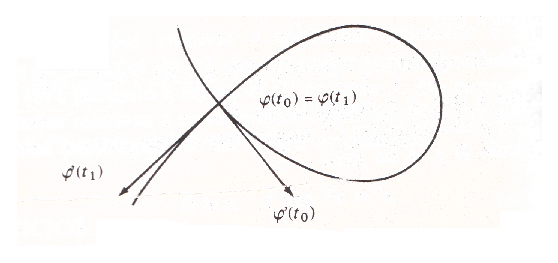
\includegraphics{dibu1.eps}
\end{center}

\emph{Sugerencia:} Notar que:
\[
    \frac{d}{dt}(t\sin t)=t\cos t+\sin t \quad\hbox{y}\quad
    \frac{d}{dt}(t^2\sin t)=t^2\cos t+2t\sin t.
\]
Sea $\varphi$ una soluci'on de \eqref{ecuacion} con
$f:\mathbb{R}\times\mathbb{R}^2\to\mathbb{R}^2$ dada por:
\[
    f(t,(x,y))=(t\cos t+\sin t, t^2\cos t +2t\sin t)
\]
y condiciones iniciales $(x(0),y(0))=(0,0)$. Calcular entonces
$\varphi(\pi)$, $\varphi(2\pi)$, $\varphi'(\pi)$ y $\varphi'(2\pi)$.

\item[c.] En caso de que \textrm{b} sea afirmativo, estudiar esto en
t'erminos de la unicidad de las soluciones dada por el Teorema
de Picard.



\item[d.] Comparar los resultados de los incisos \textrm{a} y \textrm{b}.
\end{enumerate}

\end{ejercicio}


\begin{ejercicio}   Sea
$f:\mathbb{R}\times\mathbb{R}^n\to\mathbb{R}^n$ Lipschitziana. Demostrar
que existe una soluci'on de:
\[
    \left\{%
\begin{array}{ll}
    x'=f(t,x); \\
    x(t_0)=x_0 \\
\end{array}%
\right.
\]
definida en $\mathbb{R}$.
\end{ejercicio}







\begin{ejercicio} En el rect'angulo $P=\{(t,x):|t-t_0|<a,
|x-x_0|<b\}\subset\mathbb{R}^2$, sean $f,g$ dos funciones continuas y
localmente lipschitzianas. Si $f<g$ en $P$ entonces para $\psi$ y
$\varphi$ soluciones de
\[
    x'=g(t,x),x(t_0)=x_0\quad\hbox{y}\quad x'=f(t,x),x(t_0)=x_0
\]
respectivamente, definidas en $0\leq t\leq c$,
demostrar que $\varphi(t)\leq\psi(t)$  para todo $t_0<t\leq c$.
\end{ejercicio}

\begin{ejercicio} Sea $\{\varphi_n\}$ una sucesi'on de funciones
definidas por
\[
    \varphi_0(x)=0,\quad \varphi_{n}(x)=1+\int_0^x
    (\varphi_{n-1}(t))^2dt.
\]
Demostrar que $\varphi_n$ es un polinomio de grado $2^{n-1}-1$ cuyos
coeficientes est'an en $[0,1]$. Demostrar que para $|x|<1$,
$\varphi_n\to\varphi$, donde $\varphi$ es soluci'on de $y'=y^2$,
$y(0)=1$.
\end{ejercicio}

\begin{ejercicio} Sea $f(t,x)$ definida y continua en
$\Omega=\mathbb{R}\times\mathbb{R}^n$. Supongamos que
 $f(t,x)=f(t+1,x)$ y que $f$ es lipschitziana en
 $[0,1]\times\mathbb{R}^n$. Probar que toda soluci'on
 $\varphi(t,t_0,x_0)$ est'a definida para todo $t\in\mathbb{R}$ y
 $\varphi(t,t_0,x_0)=\varphi(t+1,t_0+1,x_0)$.

\end{ejercicio}

%\begin{ejercicio} Sea $H:\mathbb{R}^n\to\mathbb{R}^n$  de clase
%$C^1$. Sea $f(t,x)$ continua en $\mathbb{R}\times\mathbb{R}^n$ tal que:
%\[
%    f(t,H(x))=DH(x)\cdot f(t,x)
%\]
%para todo $(t,x)\in\mathbb{R}\times\mathbb{R}^n$. Si $f$
%es lipschitziana y $\varphi(t,t_0,x_0)$ denota una soluci'on de
%$x'=f(t,x)$ que pasa por $(t_0,x_0)$ probar que:
%\[
%    \varphi(t,t_0,H(x))=H(\varphi(t,t_0,x_0)).
%\]
%\end{ejercicio}
%
%\begin{ejercicio} Si $X=(X_1,\ldots,X_n)$ es un campo vectorial de
%clase $C^1$ en $\mathbb{R}^n$ y $V$ una funci'on real
%diferenciable en $\mathbb{R}^n$ tal que:
%\[
%    \sum\limits_{i=1}^{n}\frac{\partial V}{\partial x_i}(x)X_i\leq
%    0\quad\hbox{y}\quad V(x)\geq |x|^2
%\]
%para todo $x\in\mathbb{R}^n$, demostrar que toda soluci'on de
%$x'=X(x)$ est'a definida para todo $t>0$.
%\end{ejercicio}
%
%\begin{ejercicio} Sea $f:\mathbb{R}^2\to\mathbb{R}$ continua y localmente lipschitziana respecto a $x$.
%Supongamos que existen dos soluciones
%$\varphi_1,\varphi_2:[0,1]\to\mathbb{R}$ de $x'=f(t,x)$ que satisfacen:
%\[
%    \hbox{Graf }\varphi_1\cap\hbox{Graf }\varphi_2=\{(0,p),(1,q)\}
%\]
%y que
%\[
%    \hbox{Graf }\varphi_1\cup\hbox{Graf }\varphi_2
%\]
%es la frontera de una regi'on $D$
%homeomorfa a un c'irculo. Demostrar que para todo $x\in D$
%existe una soluci'on $\varphi$ de $x'=f(t,x)$ tal que su gr'afico
%contiene $(0,p)$, $(1,q)$ y $x$.
%
%
%\end{ejercicio}
%\begin{ejercicio} Considerar el sistema conservativo:
%\[
%    \ddot{X}=F(X),
%\]
%donde $F\subset \mathbb{R}^n\to\mathbb{R}^n$ es una funci�n de
%clase $C^1$ y $F=-\nabla V$ con $V:U\to\mathbb{R}$ de clase $C^2$.
%Considerar la energ�a total del sistema:
%\[
%    E(X,V)=\frac12|V|^2+V(X).
%\]
%Demostrar que si, para cierto $(X_0,V_0)$ la superficie de energ�a
%\[
%    S(E_0)=\{(X,V):E(X,V)=E(X_0,V_0)\}
%\]
%es compacta entonces la soluci�n m�xima que pasa por $(X_0,V_0)$
%est� definida para todo tiempo.
%\end{ejercicio}

\end{document}
